
\section{Address Spaces}

The full accessible Program memory can be accessed by \verb|PEEK|/\verb|POKE|, 
\verb|LPEEK|/\verb|LPOKE|, \verb|DPEEK|/\verb|DPOKE|. Be careful. You can
manipulate all symbols of the interpreter and or dynamically linked libraries
and your program. Address spaces belonging to other programs which are not
shared memory blocks can not be accessed. You will get a segmentation fault on
trying this.

\section{Graphics: Drawing and Painting}

A graphics window will be automatically opened when the first graphic command
appears in your program. Without using any graphic commands no X11-Server is
needed at all and your programs also runs under a text console or as a daemon
or as CGI scripts. But if you want to draw anything with e.g. \verb|LINE|,
\verb|CIRCLE| or \verb|BOX|, control the MOUSE pointer, the keyboard or use
the graphical user interface with e.g. \verb|ALERT| or \verb|MENU|, a graphic
window will open with the default geometry \verb|640x400|. All graphic output
can be done in full color which can be set with the \verb|GET_COLOR()| and the
\verb|COLOR| statements. Moreover, there can be up to 16 different graphic
windows opened at a time. Please note that all graphics is displayed after a
\verb|SHOWPAGE| command only. This allows fast animations.

To allow for animated bitmap graphics and icons, X11-Basic offers the commands
\verb|GET| and \verb|PUT|, which retrieve rectangular regions from the
graphics-window into a string or put back bitmap graphics data from the 
string to the graphics screen or window. The file format used with 
\verb|PUT| is a standard .BMP bitmap, so also externally created icons can be
used. Transparency and alpha channels are supported.


\section{Reading from and Writing to Files}

Before you may read from or write to a file, you need to open it; once you are
done, you should close it. Each open file is designated by a simple number,
which might be stored within a variable and must be supplied to the \verb|PRINT| and
\verb|INPUT| commands if you want to access the file. 

If you need more control, you may consider reading and writing one byte at a
time, using the multi-purpose commands \verb|INP()| and \verb|OUT|, or reading
the whole file as a binary block with \verb|BLOAD|.

\section{Internet connections, special files and sockets}

X11-Basic allows to connect a program to another Program on a different (or
the same) host computer via standard internet protocols or pipes. 

Basically there are two methods of connections to other computers on a network: The TCP/IP Based connections 
via streams and the implementation of a connectionless, unreliable datagram 
packet service (UDP). 

A method of passing data between two applications on the same computer is using Pipes.
Pipes are special files which are created in the local filesystem. 

\subsection{Local inter process communication: Pipes}
A pipe is a unidirectional data channel that can be used for interprocess 
communication. The UNIX kernel usually supports this mechanism. The pipe can
be used to send information or data from one process to another. Here is a little
example progam you can use to play with it:

\begin{mdframed}[hidealllines=true,backgroundcolor=blue!20]
{\footnotesize
\begin{verbatim}
PIPE #1,#2
a=FORK()
IF a=0    ! Child instance
  GPRINT "Hi, I am Child !",b
  DO
    SHOWPAGE
    LINEINPUT #1,t$
    GPRINT t$
  LOOP
  ' This instance never ends ...
ELSE IF a=-1  
  PRINT "ERROR, fork() failed !"
  QUIT
ELSE      ! parent instance
  DO
    DUMP
    ALERT 1,"Hi, I am Parent. Child PID="+str$(a),1," OK | Kill Child ! ",b
    DUMP
    PRINt #2,SYSTEM$("date")
    FLUSH #2
    IF b=2
      SYSTEM "kill "+str$(a)
      ALERT 1,"Child PID="+str$(a)+" killed !",1," OK ",b
      QUIT
    ENDIF
  LOOP
ENDIF
QUIT
\end{verbatim} }
\end{mdframed}
Instad of with pipes, the interprocess communication can also be done using a
shared memory segment.


\subsection{World-Wide communication: Sockets}

Most inter-process communication uses the client server model. These terms refer
to the two processes which will be communicating with each other. One of the
two processes, the client, connects to the other process, the server, typically
to make a request for information. A good analogy is a person who makes a phone
call to another person.

Notice that the client needs to know of the existence of and the address of the
server, but the server does not need to know the address of (or even the
existence of) the client prior to the connection being established. Notice also
that once a connection is established, both sides can send and receive
information.

When a socket is created, the program has to specify the address domain and the
socket type. Two processes can communicate with each other only if their
sockets are of the same type and in the same domain. There are two widely used
address domains, the Unix domain, in which two processes which share a common
file system communicate, and the Internet domain, in which two processes
running on any two hosts on the Internet communicate. Each of these has its own
address format.

The address of a socket in the Unix domain is a character string which is
basically an entry in the file system.

The address of a socket in the Internet domain consists of the Internet address
of the host machine (every computer on the Internet has a unique 32 bit
address, often referred to as its IP address). In addition, each socket needs a
port number on that host. Port numbers are 16 bit unsigned integers. The lower
numbers are reserved in Unix for standard services. For example, the port
number for the FTP server is 21. It is important that standard services be at
the same port on all computers so that clients will know their addresses.
However, port numbers above 2000 are generally available.


\paragraph{Socket Types}


There are two widely used socket types, stream sockets, and datagram sockets.
Stream sockets treat communications as a continuous stream of characters, while
datagram sockets have to read entire messages at once. Each uses its own
communications protocol. Stream sockets use TCP (Transmission Control
Protocol), which is a reliable, stream oriented protocol, and datagram sockets
use UDP (Unix Datagram Protocol), which is unreliable and message oriented.



\paragraph{TCP/IP}

Transmission Control Protocol (TCP) provides a reliable byte-stream transfer
service between two endpoints on an internet. TCP depends on IP to move packets
around the network on its behalf. IP is inherently unreliable, so TCP protects
against data loss, data corruption, packet reordering and data duplication by
adding checksums and sequence numbers to transmitted data and, on the receiving
side, sending back packets that acknowledge the receipt of data.

Before sending data across the network, TCP establishes a connection with the
destination via an exchange of management packets. The connection is destroyed,
again via an exchange of management packets, when the application that was using
TCP indicates that no more data will be transferred. 

TCP has a multi-stage flow-control mechanism which continuously adjusts the
sender's data rate in an attempt to achieve maximum data throughput while
avoiding congestion and subsequent packet losses in the network. It also
attempts to make the best use of network resources by packing as much data as
possible into a single IP packet.

The system calls for establishing a connection are somewhat different for the
client and the server, but both involve the basic construct of a socket. A
socket is one end of an inter-process communication channel. The two processes
each establish their own socket.

The steps involved in establishing a socket on the client side are as follows:

\begin{enumerate}
   \item Create a socket with the OPEN command providing a port number
\begin{mdframed}[hidealllines=true,backgroundcolor=blue!20]
\begin{verbatim}
  OPEN "US",#1,"client",5000
\end{verbatim}\end{mdframed}
   \item Connect the socket to the address of the server using the CONNECT command
\begin{mdframed}[hidealllines=true,backgroundcolor=blue!20]
\begin{verbatim}
  CONNECT #1,"ptbtime1.ptb.de",13
\end{verbatim}\end{mdframed}
\item Instead of using Steps 1 and 2, you can alternatively use the combined
 command:
\begin{mdframed}[hidealllines=true,backgroundcolor=blue!20]
\begin{verbatim}
  OPEN "UC",#2,"ptbtime1.ptb.de",13
\end{verbatim}\end{mdframed}
   \item Send and receive data. There are a number of ways to do this, but the 
   simplest is to use the PRINT, SEND, WRITE, READ, RECEIVE INPUT commands. 
\begin{mdframed}[hidealllines=true,backgroundcolor=blue!20]
\begin{verbatim}
  PRINT #2,"GET /index.html"
  FLUSH #2
  WHILE INP?(#2)
    LINEINPUT #2,t$
    PRINT "got: ";t$
  WEND
\end{verbatim}\end{mdframed}
 \item close the connection with
\begin{mdframed}[hidealllines=true,backgroundcolor=blue!20]
\begin{verbatim}
 CLOSE #1
\end{verbatim}\end{mdframed}
\end{enumerate}

The steps involved in establishing a socket on the server side are as follows:

\begin{enumerate}
   \item Create a socket with the OPEN command and bind the socket to a port 
   number on the host machine.
\begin{mdframed}[hidealllines=true,backgroundcolor=blue!20]
\begin{verbatim}
  OPEN "US",#1,"server",5000
\end{verbatim}\end{mdframed}
   \item Listen for connections and
   \item Accept a connection with this other OPEN command, which opens 
   a connection to the connected client: 
\begin{mdframed}[hidealllines=true,backgroundcolor=blue!20]
\begin{verbatim}
  OPEN "UA",#2,"",1
\end{verbatim}\end{mdframed}
   This call typically blocks until a client connects with the server.
   \item Send and receive data on the accepted connection
\begin{mdframed}[hidealllines=true,backgroundcolor=blue!20]
\begin{verbatim}
  PRINT #2,"Welcome to X11-Basic test-server ..."
  FLUSH #2
  DO
    IF INP?(#2)
      LINEINPUT #2,t$
      PRINT "got: ";t$
    ENDIF
    EXIT IF t$="quit"
  LOOP
  PRINT #2,"goodbye..."
  FLUSH #2
\end{verbatim}\end{mdframed}
 \item close the established connection with
\begin{mdframed}[hidealllines=true,backgroundcolor=blue!20]
\begin{verbatim}
 CLOSE #2
\end{verbatim}\end{mdframed} and listen to the next connection (folow step 3) or 
 \item close the socket if not further needed.
\begin{mdframed}[hidealllines=true,backgroundcolor=blue!20]
\begin{verbatim}
 CLOSE #1
\end{verbatim}\end{mdframed}
\end{enumerate}

\paragraph{UDP}
 
User Datagram Protocol (UDP) provides an unreliable packetized data transfer
service between endpoints on a network. 

First, a socket has to be crated with the OPEN command:

\begin{mdframed}[hidealllines=true,backgroundcolor=blue!20]
\begin{verbatim}
  OPEN "UU",#1,"sender",5556
\end{verbatim}
\end{mdframed}

When a UDP socket is created, its local and remote addresses are
unspecified. Datagrams can be sent immediately using SEND with a valid
destination address and port as argument:
\begin{mdframed}[hidealllines=true,backgroundcolor=blue!20]
{\footnotesize\linespread{0.8}\begin{verbatim}
SEND #1,"This is my message",CVL(CHR$(131)+CHR$(195)+CHR$(15)+CHR$(200)),5000
\end{verbatim}}
\end{mdframed}
   
UDP uses the IPv4 address format, so a long integer has to be passed.

When CONNECT is called on the socket the default destination address is set and
datagrams can now be sent using SEND without specifying an destination address.
It is still possible to send to other destinations by passing an address to
SEND.

\begin{mdframed}[hidealllines=true,backgroundcolor=blue!20]
\begin{verbatim}
CONNECT #1,"localhost",5555
SEND #1,"This is my message"
\end{verbatim}
\end{mdframed}

All receive operations return only one packet.
       
\begin{mdframed}[hidealllines=true,backgroundcolor=blue!20]
\begin{verbatim}
IF INP?(#1)
  RECEIVE #1,t$,adr
  PRINT "Received Message: ";t$;" from ";HEX$(adr)
ENDIF
\end{verbatim}
\end{mdframed}

INP?(\#n) Returns the size of the next pending datagram in bytes, or 0 when no
datagram is pending.

The Socket should be closed when the connection is not goint to be used any more:
\begin{mdframed}[hidealllines=true,backgroundcolor=blue!20]
\begin{verbatim}
CLOSE #1
\end{verbatim}
\end{mdframed}

UDP does not guarantee to actually deliver the data to the destination, nor does
it guarantee that data packets will be delivered to the destination in the order
in which they were sent by the source, nor does it guarantee that only one copy
of the data will be delivered to the destination. UDP does guarantee data
integrity, and it does this by adding a checksum to the data before
transmission. 

\section{Accessing USB devices}

X11-Basic has a builtin USB interface, which allows X11-Basic programs to accedd USB-Devices, which are connected
to the computer. The interface is on a near hardware level, so the driver for the specific hardware connected must be written in 
X11-Basic. Hence, it is well possible to use dataloggers and USB-to-RS232 adapters with this methods. In pronciple every USB-Device 
can be accessed, if the protocol for data transfers and data interpretation is known. 

Please see the example program \verb|usb.bas| for an example, how to readout data from a \verb|VOLTCRAFT VDTL101-T| datalogger.

USB support is work in progress and may not yet work on Android and WINDOWS. 

USB-Devices are opened with the OPEN command. Instead of a filename, a combination if PID/VID is used. 
Once opened, the commands CLOSE, IOCTL(), SEND and RECEIVE can be used on that device. 
(PRINT and INPUT currently will not work).


\section{Data within the program}

You may store data within your program within DATA-statements; during execution
you will probably want to READ it into variables or arrays. Also the assignment
of constant to arrays may be used to store data in your program and last but not
least the \verb|INLINE$()| function may be used to store huge binary data
segments.

The first example shows how to store conventional data (numbers and strings)
within the sourcecode of a basic program:

\begin{mdframed}[hidealllines=true,backgroundcolor=blue!20]
\begin{verbatim}
' example how to use the DATA statement

RESTORE mydata
READ name$,age,address$,code

mydata:
DATA "Bud Spencer",30,"Holywood Street",890754
DATA "Hannelore Isendahl",15,"Max-Planck-Allee",813775
\end{verbatim}
\end{mdframed}

The following example shows how to store arbitrary binary data, which 
can be used e.g. to store the bitmapdata for a bitmap 
(
\includegraphics{biene.eps}). Or also for other resources like pictograms and
any other bitmap or icon.

\begin{mdframed}[hidealllines=true,backgroundcolor=blue!20]
{\footnotesize\linespread{0.8}
\begin{verbatim}
' output of inline.bas for X11-Basic 23.04.2002
' demo 104 Bytes.
demo$=""
demo$=demo$+"5*II@V%M@[4D=*9V,)5I@[4D=*9V,(IR?*IR=6Y*A:]OA*IS?F\.&IAI?J\D8ZII"
demo$=demo$+",*5M=;1I@V%P=;1I?F%OaJ]R=:\P,*5E?J\D>*)X,*9W,*AI>ZUE@+%X/F\R&JAV"
demo$=demo$+"A;1W&HXR&DL$"
a$=INLINE$(demo$)
PRINT len(a$),a$

' show a bitmap
biene$="($$43$%*<(1G,=E5Z&MD%_DVW'b*%H-^,EQ6>VTL$$$$"

CLEARW
t$=INLINE$(biene$)
COLOR GET_COLOR(65535,65535,65535)
FOR i=0 TO 40
  PUT_BITMAP t$,i*16,0,16,16
NEXT i
\end{verbatim}}
\end{mdframed}

For convenience, a program called \verb|inline.bas| shippes with X11-Basic. It does the
conversion from and compression of any binary file to ready-to-use X11-Basic
sourcecode.

%\section{Encrypting and decrypting data}

%Encryption is currently not compiled in.  

\section{Dynamic-link libraries}

A dynamic-link library (\verb|.so| ={\em shared object}) is a collection of
functions (subroutines) that can be used by programs or by other \verb|.so|'s.
A \verb|.so| function must be called, directly or indirectly, from a running
application and can not be run as a separate task.

Dynamic link libraries save memory space and reduce memory swapping. Memory is
saved, because many applications can use a single \verb|.so| simultaneously,
sharing a single copy of the \verb|.so| in memory. Another feature of 
\verb|.so|'s is the ability to change the functions in a \verb|.so| without
modifying the applications that use them, as long as the function's arguments
and return values do not change. A disadvantage to using \verb|.so|'s is that
an application depends on the existence of a separate \verb|.so| module. If the
\verb|.so| is not found, the application is terminated.

All documented functions from the shared objects of other software packages 
can be used and invoked from within yout X11-Basic program. 

X11-Basic will perform no check on the number and type of the API function
parameters.

\subsection{Using shared libraries and C functions}

Before an application can use a function from a \verb|.so| (if you want to use
your own functions written in C you have to compile them to a shared object
file), it must load the \verb|.so| explicitly using the \verb|LINK| statement.

\begin{mdframed}[hidealllines=true,backgroundcolor=blue!20]
\begin{verbatim}
LINK #n,"myfile.so"
\end{verbatim}
\end{mdframed}


The process of loading a \verb|.so| explicitly is called run-time linking. 

For instance, to use
the \verb|binit()| function from the \verb|trackit.so| library, an 
application must
include following lines of code (supposing, you want to use your own shared 
object made out of the c-code trackit.c):

\begin{mdframed}[hidealllines=true,backgroundcolor=blue!20]
\begin{verbatim}
IF NOT EXIST("./trackit.so")
  SYSTEM "gcc -O3 -shared -o trackit.so trackit.c" 
ENDIF
LINK #11,"./trackit.so"
~EXEC(SYM_ADR(#11,"binit"),L:n,L:200,L:VARPTR(x(0)),L:VARPTR(bins(0)))
\end{verbatim}
\end{mdframed}

The file \verb|trackit.c| contains:
\begin{mdframed}[hidealllines=true,backgroundcolor=black!20]
\begin{verbatim}
#include <stdlib.h>
#include <stdio.h>
#include <math.h>

void binit(int n,int dn,double *x,double *data) {
  int i,j;
  int over=0,under=0;
    for(i=0;i<n;i++) {
      j=(int)((x[i]+PI)/2/PI*dn);
      if(j<0) under++;
      else if(j>=dn) over++;
      else data[j]++;
    }  
}
\end{verbatim}
\end{mdframed}

X11-Basic applications can load up to 99 shared object files simultaneously, 
although the channel number space is shared with the open files.. 

To do this, parameter n must specify a value between 1 an 99. X11-Basic maintains
an internal table with 99 entries to store the handle of the loaded shared
object modules. These handles are necessary to unload the \verb|.so| when the
application is finished using them. 

The \verb|.so|'s are unloaded by invoking the \verb|UNLINK| command:
\begin{mdframed}[hidealllines=true,backgroundcolor=blue!20]
\begin{verbatim}  
UNLINK #11
\end{verbatim}
\end{mdframed}

X11-Basic currently allows only a float (double) type for the return value. 
This is currently a limitation for the use of the standard libraries. If you
have written the library function yourself, you could bypass this limitation by
passing pointers to variables.

The following parameter types are possible:
\begin{center}
\begin{tabular}{|c|c|}
\hline
L:  &  32-bits integers and pointers (long) (\%)   \\
W:  &  16-bits signed (short)  \\ 
B:  &  8-bits signed (char)  \\ 
F:  &  8 byte float (double)  \\ 
S:  &  4 byte float (float)  \\ 
\hline
\end{tabular}
\end{center}


The \verb|SYM_ADR| function determines the address of the function from its name. 
The spelling of the function name must therefore be identical to the spelling
of the function in the \verb|.so|. 

When passing the address of the string, a null byte must be added to the
end of the string. 


\section{Memory management}

Normally, X11-Basic takes care of most of the memory management for the
programmer. When a variable, string or array is declared, X11-Basic
allocates the required memory and releases it when the application is
terminated. However, there may be situations when a programmer wants to
allocate additional memory. 

\subsection{Allocating memory}

If an application needs to store small amounts of memory, it should use
strings. 
Strings are often used as a buffer for functions. 
The address of the memory occupied by a string can be obtained by the 
\verb|VARPTR()| function. Its length by the \verb|LEN()| function.


To allocate memory from the global and system-wide program user space 
memory pool you might use the function
\verb|MALLOC()|. For instance, to allocate 2000 bytes, you might use:

\begin{mdframed}[hidealllines=true,backgroundcolor=blue!20]
\begin{verbatim}
ptr%=MALLOC(2000)
\end{verbatim}
\end{mdframed}

A global memory block allocated with \verb|MALLOC| must be freed using the 
\verb|FREE()|
function. An application should always free all memory blocks before
exiting. For instance:
\begin{mdframed}[hidealllines=true,backgroundcolor=blue!20]
\begin{verbatim}
FREE Ptr% 
\end{verbatim}
\end{mdframed}

\section{Other features}
\begin{itemize}
  \item X11-Basic programs may start other programs with the commands 
        \verb|SYSTEM| and \verb|SYSTEM$()|.
  \item The \verb|ENV$()| function allows access to environment variables.
  \item The current time or date can be retrieved with 
        \verb|TIME$| and \verb|DATE$|.
  \item The interpreter allows self modifying code. 
  \item It is possible to link shared library objects and use the functions 
        provided from within the X11-Basic program 
\end{itemize}


\chapter{Graphical User Interface}

This chapter describes how to use the graphical user interface (GUI) built into
X11-Basic.

\section{ALERT and FILESELECT}

Two most often used graphic functions are implemented as a full functional
graphical user interface dialog: Message boxes and a file selector.
Arbitrary dialogs can be created with the object and resource functions. 
Also a pull down menu function is implemented.

\begin{SCfigure}
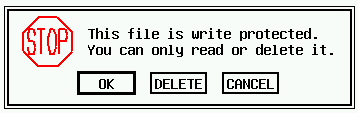
\includegraphics[width=0.5\textwidth]{alert1.eps}
\caption{A message box.}
\label{alert1}
\end{SCfigure}

Fig.~\ref{alert1} shows a typical messagebox. 
The command which produces it is:
\begin{mdframed}[hidealllines=true,backgroundcolor=blue!20]
\begin{verbatim}
ALERT 3,"This file is write protected.|You can only read or \
         delete it.",1,"OK|DELETE|CANCEL",sel
\end{verbatim}
\end{mdframed}

ALERT boxes can also be used to manage simple input forms 
like the one you can see in fig.~\ref{alert3}. 
Here is a little example program:
\begin{mdframed}[hidealllines=true,backgroundcolor=blue!20]
\begin{verbatim}
CLEARW 
i=1
name$="TEST01"
posx$="N54�50'32.3"
posy$="E007�50'32.3"
t$="Edit waypoint:||Name:   "+CHR$(27)+name$+"|"
t$=t$+"Breite: "+chr$(27)+posx$+"|"
t$=t$+"L�nge:  "+chr$(27)+posy$+"|"
t$=t$+"H�he:   "+chr$(27)+str$(alt,5,5)+"|"
t$=t$+"Typ:    "+chr$(27)+hex$(styp,4,4)+"|" 
ALERT 0,t$,1,"OK|UPDATE|L�SCHEN|CANCEL",a,f$
WHILE LEN(f$)
  WORT_SEP f$,CHR$(13),0,a$,f$
  PRINT "Feld";i;": ",a$
  INC i
WEND
QUIT
\end{verbatim}
\end{mdframed}

\begin{SCfigure}
  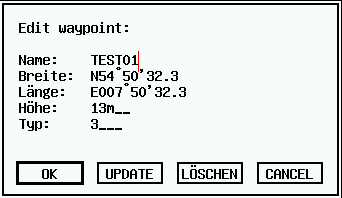
\includegraphics[width=0.5\textwidth]{alert3.eps}
  \caption{A simple input box.}
  \label{alert3}
\end{SCfigure}


\begin{SCfigure}
  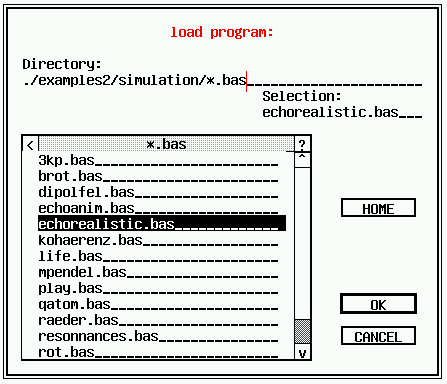
\includegraphics[width=0.7\textwidth]{fileselect.eps}
  \caption{The fileselecetor}
  \label{filesel}
\end{SCfigure}
Fig.~\ref{filesel} shows the fileselector box. The command which produces it is:
\begin{mdframed}[hidealllines=true,backgroundcolor=blue!20]
\begin{verbatim}
FILESELECT "load program:","./*.bas","in.bas",f$
\end{verbatim}
\end{mdframed}

The complete path and filename of the selected file will be returned in 
\verb|f$|.


\begin{SCfigure}
  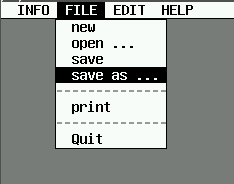
\includegraphics[width=0.3\textwidth]{menu.eps}
  \caption{A pull down menu}
  \label{filesel}
\end{SCfigure}


\section{Resources}

X11-Basic resources consist of object trees, strings, and bitmaps used by a
basic program. They encapsulate the user interface and make internationalization
easier by placing all program strings in a single file. The data format of
X11Basic resource is downwards compatible with the Atari-ST GEM implementation.

\begin{figure}
\begin{center}

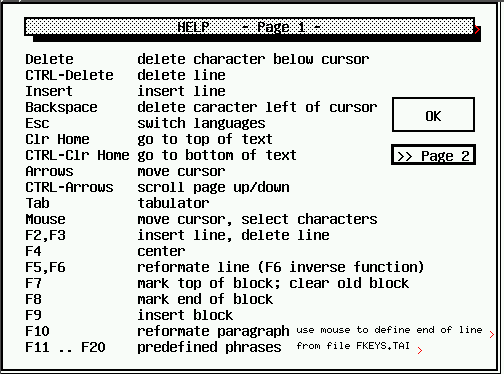
\includegraphics[width=0.48\textwidth]{form1.eps}
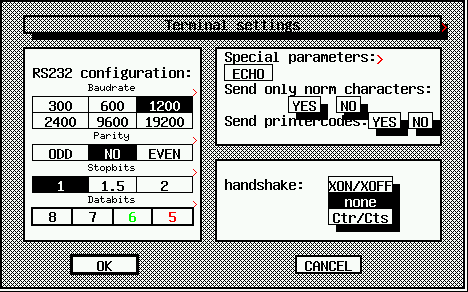
\includegraphics[width=0.48\textwidth]{form2.eps}
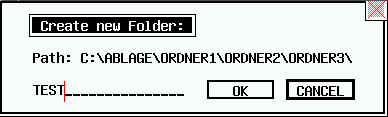
\includegraphics[width=0.48\textwidth]{form3.eps}
\end{center}
\caption{Examples of forms in X11-Basic}
\label{form1}
\end{figure}



Resources are generally created using a Resource Construction
Set (RCS) and saved to a \verb|.RSC| file which is loaded by 
\verb|RSRC_LOAD()| at program initialization time.

Resources may also be embedded as data structures in source code (the 
utility programs \verb|rsc2gui.bas| and \verb|gui2bas.bas| convert \verb|.RSC| files to 
source code). 
Resources contain pointers and coordinates which must be fixed up
before being used.
\verb|RSRC_LOAD()| does this automatically, however if you use an embedded
resource you must take care of this by yourself on each object in each object
tree to convert the initial character coordinates of to screen coordinates.
This allows resources designed on screens with different aspect ratios and
system fonts to appear the same. 
Once a resource is loaded use \verb|rsrc_gaddr()| to obtain pointers to
individual object trees which can then be manipulated directly or with the 
X11-Basic built-in functions. 

\subsection{Objects}

Objects can be boxes, buttons, text, images, and more. An object tree
is an array of OBJECT structures linked to form a structured
relationship to each other. The object itself is a section of data 
which can be held by a string in X11-Basic.

The OBJECT structure is format is as follows:

\begin{verbatim}
object$=MKI$(ob_next)+MKI$(ob_head)+MKI$(ob_tail)+
        MKI$(ob_type)+MKI$(ob_flags)+MKI$(ob_state)+
        MKL$(ob_spec)+MKI$(ob_x)+MKI$(ob_y)+MKI$(ob_width)+
        MKI$(ob_height)
\end{verbatim}

An Object tree is a collection of objects:

\begin{verbatim}
tree$=object0$+object1$+ ... +objectn$
\end{verbatim}

The first object in an OBJECT tree is called the ROOT object (OBJECT 0). It's
coordinates are relative to the upper-left hand corner of the graphics window. 
The ROOT object can have any number of children and each child can have
children of their own. In each case, the OBJECT's coordinates, \verb|ob_x|,
\verb|ob_y|, \verb|ob_width|, and \verb|ob_height| are relative to that of its
parent. The X11-Basic function \verb|objc_offset()| can, however, be used to
determine the exact screen coordinates of a child object. \verb|objc_find()| is
used to determine the object at a given screen coordinate.

The \verb|ob_next|, \verb|ob_head|, and \verb|ob_tail| fields determine this
relationship between parent OBJECTs and child OBJECTs.

\begin{description}

\item[ob\_next] the index (counting objects from the first object in the
object tree) of the object's next sibling at the same level in the object tree
array. The ROOT object should set this value to -1. The last child at any given
nesting level should set this to the index of its parent.

\item[ob\_head] the index of the first child of the current object. If the
object has no children then this value should be -1. 

\item[ob\_tail] the index of the last child: the tail of the list of the
object's children in the object tree array If the object has no children then
this value should be -1.

\item[ob\_type] the object type. The low byte of the ob\_type field 
specifies the object type as follows:

\begin{center}\begin{longtable}{|cll|}
\hline
{\bf ob\_type} & {\bf Name} & {\bf Description}\\
\hline
  20 &  G\_BOX	    &   Box		\\	    
  21 &  G\_TEXT	    &   Formatted Text  \\	    
  22 &  G\_BOXTEXT   &   Formatted Text in a Box \\
  23 &  G\_IMAGE     &   Monochrome Image	\\    
  24 &  G\_PROGDEF   &   Programmer-Defined Object\\
  25 &  G\_IBOX	    &   Invisible Box		  \\  
  26 &  G\_BUTTON    &   Push Button w/String	   \\ 
  27 &  G\_BOXCHAR   &   Character in a Box	   \\ 
  28 &  G\_STRING    &   Un-formatted Text	   \\ 
  29 &  G\_FTEXT     &   Editable Formatted Text \\
  30 &  G\_FBOXTEXT  &   Editable Formatted Text in a Box\\
  31 &  G\_ICON	    &   Monochrome Icon \\
  32 &  G\_TITLE     &   Menu Title\\
  33 &  G\_CICON     &   Color Icon \\
\hline
\end{longtable}\end{center}

\item[ob\_flags] The ob\_flags field of the object structure is a bitmask of
different flags that can be applied to any object. You may want to apply 
one ore more flags at once. Just add the values ob\_flags.

\begin{center}\begin{longtable}{|clp{9cm}|}
\hline
{\bf ob\_flags} & {\bf Name} & {\bf Description}\\
\hline
0 & NONE       & No flag \\\hline
1 & SELECTABLE & object is selected. state may be toggled by clicking on it with the mouse.\\\hline
2 & DEFAULT    & An EXIT object with this bit set will have a thicker outline and be triggered when the 
                 user presses return.\\\hline
4 & EXIT       & Clicking on this OBJECT and releasing the mouse button while still over it 
                 will cause the dialog to exit.\\\hline
8 & EDITABLE   & Set for FTEXT and FBOXTEXT objects to indicate that they may receive edit focus.\\\hline
16 & RBUTTON   & This object is one of a group of radio buttons. Clicking on it will deselect
                 any selected objects at the same tree level that also have the RBUTTON flag
                 set. Likewise, it will be deselected automatically when any other object is selected.\\\hline
32 & LASTOB    & This flag signals that the current OBJECT is the last in the object tree. (Required!)\\\hline
64 & TOUCHEXIT & Setting this flag causes the OBJECT to return an exit state immediately after   
                 being clicked on with the mouse.\\\hline
256 & HIDETREE & This OBJECT and all of its children will not be drawn.\\\hline
512 & INDIRECT & This flag cause the ob\_spec field to be interpreted as a pointer to the      
                 ob\_spec value rather than the value itself.\\\hline
1024 & FL3DIND & Setting this flag causes the OBJECT to be drawn as a 3D indicator. This is  
                 appropriate for radio and toggle buttons.\\\hline
2048 & FL3DACT & Setting this flag causes the OBJECT to be drawn as a 3D activator. This is  
                 appropriate for EXIT buttons.\\\hline
3072 & FL3DBAK & If these bits are set, the object is treated as an AES background object.  
                 If it is OUTLINED, the outlined is drawn in a 3D manner. If its color
                 is set to WHITE and its fill pattern is set to 0 then the OBJECT will inherit 
                 the default 3D background color.\\\hline
4096 & SUBMENU & This bit is set on menu items which have a sub-menu attachment. This bit also
                 indicates that the high byte of the ob\_type field is being used by the menu
                 system.\\\hline
\end{longtable}\end{center}

\item[ob\_state] The ob\_state field determines the display state of the object as
follows:

\begin{center}\begin{longtable}{|clp{9cm}|}
\hline
{\bf ob\_state} & {\bf Name} & {\bf Description}\\
\hline
0 & NORMAL   & Normal state \\\hline
1 & SELECTED & The object is selected. An object with this bit set will be drawn in inverse
               video except for G\_CICON which will use its 'selected' image.\\\hline
2 & CROSSED  & An OBJECT with this bit set will be drawn over with a white cross (this   
               state can only usually be seen over a colored or	SELECTED object).\\\hline
4 & CHECKED  & An OBJECT with this bit set will be displayed with a check mark in its    
               upper-left corner.\\\hline
8 & DISABLED & An OBJECT with this bit set will ignore user input. Text objects with this   
               bit set will draw in grey or a dithered pattern.\\\hline
16 & OUTLINED & G\_BOX, G\_IBOX, G\_BOXTEXT, G\_FBOXTEXT, and G\_BOXCHAR OBJECTs   
               with this bit set will be drawn with a double border.\\\hline
32 & SHADOWED & G\_BOX, G\_IBOX, G\_BOXTEXT, G\_FBOXTEXT, and G\_BOXCHAR OBJECTs   
                will be drawn with a shadow.\\\hline
\end{longtable}\end{center}

\item[ob\_spec] The Object-Specific Field

The ob\_spec field contains different data depending on the object type
as indicated in the table below:
\begin{center}\begin{longtable}{|lp{9cm}|}
\hline
G\_BOX &
The low 16 bits contain a WORD containing color information for the OBJECT. 
Bits 23-16 contain a signed BYTE representing the border thickness of the 
box.\\\hline
G\_TEXT &The ob\_spec field contains a pointer to a TEDINFO  structure. \\\hline  
G\_BOXTEXT &The ob\_spec field contains a pointer to a TEDINFO structure.   \\\hline
G\_IMAGE   & The ob\_spec field points to a BITBLK structure. \\\hline
G\_PROGDEF & The ob\_spec field points to a APPLBLK structure.\\\hline
G\_IBOX	  & The low 16 bits contain a WORD containing color information for the OBJECT. 
Bits 23-16 contain a signed BYTE representing the border thickness of the box.\\\hline
G\_BUTTON  & The ob\_spec field contains a pointer to the text to be contained in the button.\\\hline
G\_BOXCHAR & The low 16 bits contain a WORD containing color information for the OBJECT. 
Bits 23-16 contain a signed BYTE representing the border thickness of the box. 
Bits 31-24 contain the ASCII value of the character to display.\\\hline
G\_STRING  & The ob\_spec field contains a pointer to the text to be displayed.\\\hline
G\_FTEXT   & The ob\_spec field contains a pointer to a TEDINFO structure.\\\hline
G\_FBOXTEXT & The ob\_spec field contains a pointer to a TEDINFO structure.\\\hline
G\_ICON & The ob\_spec field contains a pointer to an ICONBLK structure. \\\hline    
G\_TITLE  & The ob\_spec field contains a pointer to the text to be used for the title.\\\hline
G\_CICON  & The ob\_spec field contains a pointer to a CICONBLK structure.\\\hline
\end{longtable}\end{center}

\begin{description}
\item[objc\_colorword]
Almost all objects reference a WORD containing the object color as
defined below.

{\footnotesize
\begin{verbatim}
objc_colorword=bbbbcccctpppcccc

Bits 15-12 contain the border color 
Bits 11-8  contain the text color 
Bit   7    is 1 if opaque or 0 if transparent 
Bits 6-4   contain the fill pattern index 
Bits 3-0   contain the fill color 
\end{verbatim}}

Available colors for fill patterns, text, and borders are listed
below:
\begin{center}
\begin{tabular}{|cll|}
\hline
{\bf Value} &{\bf  Name}&{\bf  Color}  \\
\hline
 0&  WHITE	&  White\\
 1&  BLACK	&  Black\\
 2&  RED	&  Red\\
 3&  GREEN	&  Green\\
 4&  BLUE	&  Blue\\
 5&  CYAN	&  Cyan\\
 6&  YELLOW	&  Yellow\\
 7&  MAGENTA	&  Magenta\\
 8&  LWHITE	&  Light Gray\\
 9&  LBLACK	&  Dark Gray\\
 10& LRED	&  Light Red\\
 11& LGREEN	&  Light Green\\
 12& LBLUE	&  Light Blue\\
 13& LCYAN	&  Light Cyan\\
 14& LYELLOW	&  Light Yellow\\
 15& LMAGENTA	&  Light Magenta\\
\hline
\end{tabular}
\end{center}


\item[TEDINFO]
G\_TEXT, G\_BOXTEXT, G\_FTEXT, and G\_FBOXTEXT objects all reference a
TEDINFO structure in their ob\_spec field. The TEDINFO structure is
defined below:
 {\footnotesize
\begin{verbatim}                                                         
tedinfo$=MKL$(VARPTR(te_ptext$))+MKL$(VARPTR(te_ptmplt$))+
         MKL$(VARPTR(te_pvalid$))+MKI$(te_font)+MKI$(te_fontid)+
         MKI$(te_just)+MKI$(te_color)+MKI$(te_fontsize)+
         MKI$(te_thickness)+MKI$(te_txtlen)+MKI$(te_tmplen)
\end{verbatim}}

The three character pointer point to text strings required for 
\verb|G_FTEXT|
and \verb|G_FBOXTEXT| objects. te\_ptext points to the actual text to be
displayed and is the only field used by all text objects. te\_ptmplt
points to the text template for editable fields. For each character
that the user can enter, the text string should contain a tilde
character (ASCII 126). Other characters are displayed but cannot be
overwritten by the user. \verb|te_pvalid| contains validation characters for
each character the user may enter. The current acceptable validation
characters are:

\begin{center}
\begin{tabular}{|cl|}
\hline
{\bf Character} &{\bf  Allows}\\
\hline
9 & Digits 0-9\\
A & Uppercase letters A-Z plus space\\
a & Upper and lowercase letters plus space\\
N & Digits 0-9, uppercase letters A-Z and space\\
n & Digits 0-9, upper and lowercase letters A-Z  and space\\
F & Valid DOS filename characters plus question mark and asterisk \\
P & Valid DOS pathname characters, backslash, colon, question mark, asterisk \\
p & Valid DOS pathname characters, backslash and colon\\
X & All characters\\
\hline
\end{tabular}
\end{center}

\verb|te_font| may be set to any of the following values:

\begin{center}
\begin{tabular}{|cll|}
\hline
{\bf te\_font} &{\bf  Name} & {\bf Description} \\
\hline
3 &IBM    & Use the standard monospaced font.\\
5 &SMALL  &  Use the small monospaced font.\\
\hline
\end{tabular}
\end{center}

\verb|te_just| sets the justification of the text output as follows:

\begin{center}
\begin{tabular}{|cll|}
\hline
{\bf te\_just} &{\bf  Name} & {\bf Description} \\
\hline
0 & TE\_LEFT & Left Justify\\
1 & TE\_RIGHT & Right Justify\\
2 & TE\_CNTR & Center\\
\hline
\end{tabular}
\end{center}


te\_thickness sets the border thickness (positive and negative values
are acceptable) of the G\_BOXTEXT or G\_FBOXTEXT object. 

te\_txtlen and
te\_tmplen should be set to the length of the starting text and
template length respectively. 

\item[BITBLK]
G\_IMAGE objects contain a pointer to a BITBLK structure in their
ob\_spec field. The BITBLK structure is defined as follows:

 {\footnotesize
\begin{verbatim}                                                         
bitblk$=MKL$(VARPTR(bi_pdata$))+MKI$(bi_wb)+MKI$(bi_hl)+
        MKI$(bi_x)+MKI$(bi_y)+MKI$(bi_color)
\end{verbatim}}

\verb|bi_pdata| should contain a monochrome bit image. 
\verb|bi_wb| specifies the width (in bytes) of the image. 
All BITBLK images must be a multiple of 16 pixels wide therefore this 
value must be even.
\verb|bi_hl| specifies the height of the image in scan lines (rows). 
\verb|bi_x| and \verb|bi_y| are used as offsets into \verb|bi_pdata|. 
Any data occurring before these coordinates will be ignored. 
\verb|bi_color| is a standard color WORD
where the fill color specifies the color in which the image will be
rendered.

\item[ICONBLK]
The \verb|ob_spec| field of \verb|G_ICON| objects point to an ICONBLK structure as
defined below:

 {\footnotesize
\begin{verbatim}                                                         
iconblk$=MKL$(VARPTR(ib_pmask$))+MKL$(VARPTR(ib_pdata$))+MKL$(VARPTR(ib_ptext$))+
         MKI$(ib_char)+MKI$(ib_xchar)+MKI$(ib_ychar)+
         MKI$(ib_xicon)+MKI$(ib_yicon)+MKI$(ib_wicon)+MKI$(ib_hicon)+
	 MKI$(ib_xtext)+MKI$(ib_ytext)+MKI$(ib_wtext)+MKI$(ib_htext)
\end{verbatim}}

\verb|ib_pmask| and \verb|ib_pdata| contain the monochrome mask and 
image data respectively. \verb|ib_ptext| is a string pointer to the icon text.
\verb|ib_char| defines the icon character (used for drive icons) and the icon
foreground and background color as follows:

 {\footnotesize
\begin{verbatim}                                                         
|                              ib_char                               |
|      Bits 15-12      |      Bits 11-8       |       Bits 7-0       |
|Icon Foreground Color |Icon Background Color |ASCII Character (or 0 |
|                      |                      |  for no character).  |
\end{verbatim}}

\verb|ib_xchar| and \verb|ib_ychar| specify the location of the icon character
relative to \verb|ib_xicon| and \verb|ib_yicon|. \verb|ib_xicon| and 
\verb|ib_yicon| specify the
location of the icon relative to the \verb|ob_x| and \verb|ob_y| of the object.
\verb|ib_wicon| and \verb|ib_hicon| specify the width and height of the icon in
pixels. As with images, icons must be a multiple of 16 pixels in
width.
\verb|ib_xtext| and \verb|ib_ytext| specify the location of the text string relative
to the \verb|ob_x| and \verb|ob_y| of the object. \verb|ib_wtext| and \verb|ib_htext| specify the
width and height of the icon text area.

\item[CICONBLK]

The \verb|G_CICON| object defines its
\verb|ob_spec| field to be a pointer to a CICONBLK structure as defined
below:

 {\footnotesize
\begin{verbatim}                                                         
ciconblk$=monoblk$+MKL$(VARPTR(mainlist$))
\end{verbatim}}

\verb|monoblk| contains a monochrome icon which is rendered if a color icon
matching the display parameters cannot be found. In addition, the icon
text, character, size, and positioning data from the monochrome icon
are always used for the color one. \verb|mainlist| contains the first
CICON structure in a linked list of color icons for different
resolutions. \verb|CICON| is defined as follows:

 {\footnotesize
\begin{verbatim}                                                         
cicon$=MKI$(num_planes)+MKL$(VARPTR(col_data$))+MKL$(VARPTR(col_mask$))+
       MKL$(VARPTR(sel_data$))+MKL$(VARPTR(sel_mask$))+
       MKL$(VARPTR(cicon2$))
\end{verbatim}}

\verb|num_planes| indicates the number of bit planes this color icon
contains. \verb|col_data| and \verb|col_mask| contain the icon data and 
mask for the unselected icon respectively. Likewise, 
\verb|sel_data| and \verb|sel_mask| contain the icon data and mask for 
the selected icon. \verb|cicon2$| contains
the next color icon definition. Use \verb|MKL$(0)| if no more are available.

The GUI library searches the CICONBLK object for a color icon that has the
same number of planes in the display. If none is found, the GUI library simply
uses the monochrome icon.

\item[APPLBLK]

\verb|G_PROGDEF| objects allow programmers to define custom objects and link
them transparently in the resource. The \verb|ob_spec| field of
\verb|G_PROGDEF|
objects contains a pointer to an APPLBLK as defined below:

 {\footnotesize
\begin{verbatim}                                                         
applblk$=MKL$(SYM_ADR(#1,"function"))+MKL$(ap_parm)
\end{verbatim}}

The first is a pointer to a user-defined routine which will draw the
object. This routine must be a c-Function, which has to be linked to 
X11-basic with the LINK command. The routine will be passed a pointer to a
PARMBLK structure containing the information it needs to render the
object. The routine must be defined with stack checking off and expect
to be passed its parameter on the stack. \verb|ap_parm| is a user-defined
value which is copied into the PARMBLK structure as defined below:

{\footnotesize
\begin{verbatim}                                                         
typedef struct parm_blk {
        OBJECT          *tree;
        short            pb_obj;
        short            pb_prevstate;
        short            pb_currstate;
        short            pb_x;
        short            pb_y;
        short            pb_w;
        short            pb_h;
        short            pb_xc;
        short            pb_yc;
        short            pb_wc;
        short            pb_hc;
        long             pb_parm;
} PARMBLK;
\end{verbatim}}

\verb|tree| points to the OBJECT tree of the object being drawn. The object
is located at index \verb|pb_obj|.

The routine is passed the old \verb|ob_state| of the object in
\verb|pb_prevstate|
and the new \verb|ob_state| of the object in \verb|pb_currstate|. 
If \verb|pb_prevstate|
and \verb|pb_currstate| is equal then the object should be drawn completely,
otherwise only the drawing necessary to redraw the object from
\verb|pb_prevstate| to \verb|pb_currstate| are necessary.

\verb|pb_x|, \verb|pb_y|, \verb|pb_w|, and \verb|pb_h| give the screen 
coordinates of the object.
\verb|pb_xc|, \verb|pb_yc|, \verb|pb_wc|, and \verb|pb_hc| give the 
rectangle to clip to. \verb|pb_parm|
contains a copy of the \verb|ap_parm| value in the APPLBLK structure.
The custom routine should return a short containing any remaining
\verb|ob_state| bits you wish the GUI Library to draw over your custom object.

\end{description}

\end{description}



\subsubsection{Dialogs}

Dialog boxes are modal forms of user input. This means that no other
interaction can occur between the user and applications until the
requirements of the dialog have been met and it is exited. A normal
dialog box consists of an object tree with a BOX
as its root object and any number of other controls that accept user
input. Both alert boxes and the file selector are examples of
dialog boxes.

The \verb|form_do()| function performs the simplest method of using a dialog box. Simply
construct an OBJECT tree with at least one EXIT or TOUCHEXIT object and call
\verb|form_do()|\footnote{Before you should display the dialog box using the
{\tt objc\_draw()} function. Maybe you also want to center the dialog with 
{\tt form\_center()} and save and redraw the background 
with {\tt form\_dial()}.}. All interaction with the dialog like editable fields,
radio buttons, and selectable objects will be maintained by the 
X11-Basic library until the
user strikes an EXIT or TOUCHEXIT object.


\subsection{The gui file format}

The *.gui file format, which is basically an ASCII representation of the ATARI
ST resource files (*.rsc), can be converted to X11-Basic code, which then can
handle message boxes and forms. The converter \verb|gui2bas(1)| does this job.
For conversion of ATARI ST resource files to *.gui Files see \verb|rsc2gui(1)|.

The *.gui file consists of Lines and Blocks which specify objects and their 
hierarchical dependencies.
The generic format of such an object is:

\begin{verbatim}
label: TYPE(variables) {
 ... block ...
}
\end{verbatim}

The label is optional and gives the object a name. Depending on TYPE of the
object, one or more variables are given as a comma separated list in
brackets. 

Each object may start a block with '\{' at the end of the line. Inside this
block there might be one or more objects given which then are considered as
sub-objects of the one which opened the block. The block will be closed by a
'\}' in a single line.

\begin{mdframed}[hidealllines=true,backgroundcolor=green!20]

Example:

{\footnotesize\linespread{0.8}
\begin{verbatim}
' Little selector box  (c) Markus Hoffmann    07.2003
' convert this with gui2bas !
' as an example for the use of the gui system
' with X11-Basic

BOX(X=0,Y=0,W=74,H=14, FRAME=2, FRAMECOL=1, TEXTCOL=1, BGCOL=0, PATTERN=0, TEXTMODE=0, STATE=OUTLINED+) {
  BOXTEXT(X=2,Y=1,W=70,H=1, TEXT="Select option ...", FONT=3, JUST=2, COLOR=4513, BORDER=253, STATE=SHADOWED+)
  BOX(X=2,Y=3,W=60,H=10, FRAME=-1, FRAMECOL=1, TEXTCOL=1, BGCOL=0, PATTERN=0, TEXTMODE=0) {
    FTEXT(X=1,Y=1,W=30,H=1,COLOR=4513,FONT=3,BORDER=1,TEXT="Line 1", PTMP="_______________________________________",PVALID="XXXXXXXXXXXXXXXXXXXXXXXXXXXXXXXXXXXXXXX", FLAGS=EDITABLE)
    FTEXT(X=1,Y=2,W=30,H=1,COLOR=4513,FONT=3,BORDER=1,TEXT="", PTMP="_______________________________________",PVALID="XXXXXXXXXXXXXXXXXXXXXXXXXXXXXXXXXXXXXXX", FLAGS=EDITABLE)
    FTEXT(X=1,Y=3,W=30,H=1,COLOR=4513,FONT=3,BORDER=1,TEXT="", PTMP="_______________________________________",PVALID="XXXXXXXXXXXXXXXXXXXXXXXXXXXXXXXXXXXXXXX", FLAGS=EDITABLE)
    FTEXT(X=1,Y=4,W=30,H=1,COLOR=4513,FONT=3,BORDER=1,TEXT="", PTMP="_______________________________________",PVALID="XXXXXXXXXXXXXXXXXXXXXXXXXXXXXXXXXXXXXXX", FLAGS=EDITABLE)
    BOX(X=2,Y=6,W=50,H=3, FRAME=-1, FRAMECOL=1, TEXTCOL=1, BGCOL=1, PATTERN=5, TEXTMODE=0) { 
      BUTTON(X=2,Y=1,W=4,H=1, TEXT="ON",STATE=SELECTED, FLAGS=RADIOBUTTON+SELECTABLE,FRAME=2, FRAMECOL=1, TEXTCOL=1, BGCOL=1, PATTERN=0, TEXTMODE=0)
      BUTTON(X=8,Y=1,W=4,H=1, TEXT="OFF",FLAGS=RADIOBUTTON+SELECTABLE,FRAME=2, FRAMECOL=1, TEXTCOL=1, BGCOL=1, PATTERN=0, TEXTMODE=0)
    }
  }
  ok:	  BUTTON(X=65,Y=4,W=7,H=4, TEXT="OK", FLAGS=SELECTABLE+DEFAULT+EXIT)
  cancel: BUTTON(X=65,Y=9,W=7,H=4, TEXT="CANCEL", FLAGS=SELECTABLE+EXIT+LASTOB+)
}
\end{verbatim}
}
\end{mdframed}

\section{Menus}

Most applications use a menu bar to allow the user to navigate through program
options. In addition, future versions of X11-Basic will allow pop-up menus and
drop-down list boxes (a special form of a pop-up menu). 

Here is a simple example program, which demonstrates the handling of a drop
down menu. 

\begin{mdframed}[hidealllines=true,backgroundcolor=blue!20]
{\footnotesize\linespread{0.8}
\begin{verbatim}
' Test-program for Drop-Down-Menus
'
DIM field$(50)
FOR i=0 TO 50
  READ field$(i)
  EXIT IF field$(i)="***"
NEXT i
oh=0
field$(i)=""
DATA "INFO","  Menutest"
DATA "---------------"
DATA "- Access.1","- Access.2","- Access.3","- Access.4","- Access.5"
DATA "- Access.6",""
DATA "FILE","  new","  open ...","  save","  save as ...","--------------"
DATA "  print","--------------","  Quit",""
DATA "EDIT","  cut","  copy","  paste","----------","  help1","  helper"
DATA "  assist",""
DATA "HELP","  online help","--------------","  edifac","  editor","  edilink"
DATA "  edouard",""
DATA "***"

grau=get_color(32000,32000,32000)
color grau
pbox 0,0,640,400
MENUDEF field$(),menuaction
DO 
  pause 0.05
  MENU 
LOOP
quit

PROCEDURE menuaction(k)
  local b
  IF (field$(k)="  Quit") OR (field$(k)="  exit") 
    quit
  ELSE IF field$(k)="  online help"
    oh=not oh
    MENUSET k,4*abs(oh)
  ELSE IF field$(k)="  Menutest" 
    ~form_alert(1,"[0][---- Menutest ----||(c) Markus Hoffmann 2001|X11-Basic V.1.03][ OK ]")
  ELSE   
    PRINT "MENU selected ";k;" contents: ";field$(k)
    b=form_alert(1,"[1][--- Menutest ---||You selected item (No. "+str$(k)+"),| for which was no|function defined !][ OK |disable]")
    if b=2
      MENUSET k,8
    endif
  ENDIF
RETURN
\end{verbatim}
}
\end{mdframed}


\chapter{WEB Programming}

This chapter explains how you can use X11-Basic programs for WEB-interfacing.
Especially via the use of so-called {\bf CGI-Scripts}.  

\section{What is CGI?}

CGI stands for {\em Common Gateway Interface} --- a term you don't really need to
know. In short, CGI defines how web servers and web browsers handle information
from HTML forms on web pages. This means instead of the WEB server sending
static  web pages to the clients, it can invoke a program, typically called a
cgi-script,  to generate the page on the time the request was received. These
cgi-scripts take some action, and then send a results page back to the user's
web browser. The results page might be different every time the program is run.

And these programs can be X11-Basic programs.

\subsection{Configuration}
\begin{enumerate}
\item {\bf All X11-Basic scripts must begin} with the following statement, on the first 
line:
\begin{mdframed}[hidealllines=true,backgroundcolor=blue!20]
\begin{verbatim}
#!/usr/bin/xbasic
\end{verbatim}
\end{mdframed}

Because Unix does not map file suffixes to programs, there has to be a way to 
tell Unix that this file is a X11-Basic program, and that it is to be executed
by the X11-Basic interpreter \verb|xbasic|. This is seen before in shell
scripts, in which the first line tells Unix to execute it with one of the shell
programs. The xbasic executable, which will take this file, parse it, and
execute it, is located in the directory /usr/bin. This may be different on some
systems. If you are not sure where the xbasic executable is, type which xbasic
on the command line, and it will return you the path.

\item {\bf All scripts should be marked as executable by the system.}

Executable files are types that contain instructions for the machine or an
interpreter, such as xbasic, to execute. To mark a file as executable, you need
to alter the file permissions on the script file. There are three basic
permissions: read, write, and execute. There are also three levels of access:
owner, group, and anyone. X11-Basic files should have their permissions changed so
that you, the owner, has permission to read, write and execute your file, while
others only have permission to read and execute your file. This is done with
the following command:


\begin{mdframed}[hidealllines=true,backgroundcolor=black!20]
\begin{verbatim}
chmod 755 filename.bas
\end{verbatim}
\end{mdframed}


The number 755 is the file access mask. The first digit is your permission; it
is 7 for full access. The user and anyone settings are 5 for read and execute.

\item {\bf The very first print statement} in a X11-Basic cgi script that
returns HTML should be:

\begin{mdframed}[hidealllines=true,backgroundcolor=blue!20]
\begin{verbatim}
PRINT "Content-type: text/html"+CHR$(13)
PRINT ""+CHR$(13)
FLUSH
\end{verbatim}
\end{mdframed}

When your X11-Basic script is going to return an HTML file, you must have this
as the very first print statement in order to tell the web server that this is
an HTML file. There must be two end of line characters (CR+LF) (the additional
\verb|chr$(13)|) in order for this to work. The flush statement ensures, that
this statement is sent to the web-server. After that, you usually 
\verb|print "<HTML><BODY>"| etc.

\item {\bf End your program with \verb|quit|}

Do not use \verb|END|. Otherwise the cgi-program will remain is the servers 
memory as a zombie.

\item {\bf Always use the POST method with HTML forms}

There are 2 ways to get information from the client to the web server. The GET
method takes all of the data from the forms and concatenates it onto the end of
the URL. This information is then passed to the CGI program as an environment 
variable (\verb|QUERY_STRING|). Because the GET method has the limitation of being 1024 characters
long, it is best to use the POST method. This takes the data and sends it
along with the request to the web server, without the user seeing the ugly
strings in the URL. This information is passed to the CGI program through
standard in, which the program can easily read from. To use the POST method,
make sure that your HTML form tag has \verb|METHOD=POST| (no quotes).

\item {\bf HTML forms must reference the cgi script to be executed.}

In your FORM tag, there is an ACTION attribute. This is like the HREF attribute
for a link. It should be the URL of the CGI program you want the form data sent
to. Usually this is
\verb|ACTION="/cgi-bin/filename.bas"|

\item {\bf X11-Basic-cgi files usually go in the cgi-bin directory of your web server.}

The web server has a "root" directory. This is the highest directory your HTML
files can access. (You don't want clients to be able to snoop around your
entire system, so the rest of the system is sealed off) in
this directory, there is usually one called cgi-bin, where all the CGI programs
go. Some web service providers give each user a cgi-local directory in their
home directory where they can put their cgi scripts. If this is the case, use
this one instead. 
\end{enumerate}

\section{How it works}\index{CGI|bb}

When a user activates a link to a gateway script, input is sent to the server.
The server formats this data into environment variables and checks to see
whether additional data was submitted via the standard input stream.

\subsection{Environment Variables}\index{Environment Variables}

Input to CGI scripts is usually in the form of environment variables. The
environment variables passed to gateway scripts are associated with the browser
requesting information from the server, the server processing the request, and
the data passed in the request. Environment variables are case-sensitive and are
normally used as described in this section. The standard (and platform
independent) environment variables are shown in the following table:

\begin{center}
\begin{longtable}{|l|p{10cm}|}
\hline
{\bf Variable} & {\bf Purpose}\\
\hline
\verb|AUTH_TYPE| & 
Specifies the authentication method and is used to validate a user's access.
\\\hline
\verb|CONTENT_LENGTH| & Used to provide a way of tracking the length of the 
data string as a numeric value.\\\hline
\verb|CONTENT_TYPE| & Indicates the MIME type of data. \\\hline
\verb|GATEWAY_INTERFACE| & Indicates which version of the CGI standard the 
server is using.\\\hline
\verb|HTTP_ACCEPT|	& Indicates the MIME content types the browser will accept, 
as passed to the gateway script via the server.\\\hline
\verb|HTTP_USER_AGENT| & Indicates the type of browser used to send the request, 
as passed to the gateway script via the server.\\\hline
\verb|PATH_INFO| & Identifies the extra information included in the URL after 
the identification of the CGI script. \\\hline
\verb|PATH_TRANSLATED| & Set by the server based on the PATH\_INFO variable. 
The server translates the PATH\_INFO variable into this variable. \\\hline
\verb|QUERY_STRING| & Set to the query string (if the URL contains a query string).\\\hline 
\verb|REMOTE_ADDR| & Identifies the Internet Protocol address of the remote computer making the request.\\\hline 
\verb|REMOTE_HOST| & Identifies the name of the machine making the request.\\\hline 
\verb|REMOTE_IDENT| & Identifies the machine making the request.\\\hline 
\verb|REMOTE_USER| & Identifies the user name as authenticated by the user.\\\hline 
\verb|REQUEST_METHOD| & Indicates the method by which the request was made. \\\hline 
\verb|SCRIPT_NAME| & Identifies the virtual path to the script being executed.\\\hline 
\verb|SERVER_NAME| & Identifies the server by its host name, alias, or IP address.\\\hline 
\verb|SERVER_PORT| & Identifies the port number the server received the request on.\\\hline
\verb|SERVER_PROTOCOL| & Indicates the protocol of the request sent to the server.\\\hline
%\verb|SERVER_SOFTWARE| & Identifies the Web server software.\\\hline
\end{longtable}
\end{center}
\begin{description}

\item[AUTH\_TYPE]

The \verb|AUTH_TYPE| variable provides access control to protected areas of
the Web server and can be used only on servers that support user
authentication. If an area of the Web site has no access control, the
\verb|AUTH_TYPE| variable has no value associated with it. If an area of the
Web site has access control, the \verb|AUTH_TYPE| variable is set to a specific
value that identifies the authentication scheme being used. e.g. "Basic".

Using this mechanism, the server can challenge a client's request and the
client can respond. To do this, the server sets a value for the
\verb|AUTH_TYPE| variable and the client supplies a matching value. The next
step is to authenticate the user. Using the basic authentication scheme, the
user's browser must supply authentication information that uniquely
identifies the user. This information includes a user ID and password.


\item[CONTENT\_LENGTH]

The \verb|CONTENT_LENGTH| variable provides a way of tracking the length of the
data string. This variable tells the client and server how much data to read on
the standard input stream. The value of the variable corresponds to the number
of characters in the data passed with the request. If no data is being passed,
the variable has no value.


\item[CONTENT\_TYPE]

The \verb|CONTENT_TYPE| variable indicates the data's MIME type. This
variable is set only when attached data is passed using the standard input
or output stream. The value assigned to the variable identifies the basic MIME
type and subtype as follows:
\begin{center}
\begin{longtable}{|l|p{10cm}|}
\hline
{\bf Type} & {\bf Description}\\
\hline
\verb|application| & Binary data that can be executed or used with another 
application\\\hline
\verb|audio| & A sound file that requires an output device to preview\\\hline
\verb|image| & A picture that requires an output device to preview\\\hline
\verb|message| & An encapsulated mail message\\\hline
\verb|multipart| & Data consisting of multiple parts and possibly many data 
types\\\hline
\verb|text| & Textual data that can be represented in any character set or formatting language\\\hline
\verb|video| & A video file that requires an output device to preview\\\hline
\verb|x-world|   & Experimental data type for world files\\\hline
\end{longtable}
\end{center}

MIME subtypes are defined in three categories: primary, additionally defined,
and extended. The primary subtype is the primary type of data adopted for use
as a MIME content type. Additionally defined data types are additional subtypes
that have been officially adopted as MIME content types. Extended data types
are experimental subtypes that have not been officially adopted as MIME content
types. You can easily identify extended subtypes because they begin with the
letter x followed by a hyphen. The following Table lists common MIME types and
their descriptions.
\begin{center}
\begin{longtable}{|l|p{8cm}|}
\hline
{\bf Type/Subtype} & {\bf Description}\\\hline 
\verb|application/octet-stream| & Binary data that can be executed or used with another application\\\hline 
\verb|application/pdf| & ACROBAT PDF document\\\hline 
\verb|application/postscript| & Postscript-formatted data\\\hline
\verb|application/x-compress| & Data that has been compressed using UNIX 
compress\\\hline
%\verb|application/x-dvi| & Device-independent file\\\hline 
\verb|application/x-gzip| & Data that has been compressed using UNIX gzip\\\hline
%\verb|application/x-latex| & LATEX document\\\hline
\verb|application/x-tar| & Data that has been archived using UNIX tar\\\hline
%\verb|audio/basic| & Audio in a nondescript format\\\hline
\verb|audio/x-wav| & Audio in Microsoft WAV format\\\hline
\verb|image/gif| & Image in gif format\\\hline
\verb|image/jpeg| & Image in JPEG format\\\hline
\verb|image/tiff| & Image in TIFF format\\\hline
%\verb|image/x-portable-bitmap| & Portable bitmap\\\hline
%\verb|image/x-portable-graymap| & Portable graymap\\\hline
%\verb|image/x-portable-pixmap| & Portable pixmap\\\hline
%\verb|image/x-xbitmap| & X-bitmap\\\hline
%\verb|image/x-xpixmap| & X-pixmap\\\hline
%\verb|message/external-body| & Message with external data source\\\hline
%\verb|message/partial| & Fragmented or partial message\\\hline
%\verb|message/rfc822| & RFC 822-compliant message\\\hline 
%\verb|multipart/alternative| & Data with alternative formats\\\hline
%\verb|multipart/digest| & Multipart message digest\\\hline
\verb|multipart/mixed| & Multipart message with data in multiple formats\\\hline
%\verb|multipart/parallel| & Multipart data with parts that should be viewed simultaneously\\\hline
\verb|text/html| & HTML-formatted text\\\hline
\verb|text/plain| & Plain text with no HTML formatting included\\\hline
\verb|video/mpeg| & Video in the MPEG format\\\hline
%\verb|video/x-msvideo| & Video in the Microsoft AVI format\\\hline
\end{longtable}
\end{center}
Note, that there are more than the above listed types.

Some MIME content types can be used with additional parameters. These content
types include text/plain, text/html, and all multi-part message data. The
charset parameter, which is optional, is used with the text/plain type to
identify the character set used for the data. If a charset is not specified, the
default value charset=us-ascii is assumed. Other values for charset include any
character set approved by the International Standards Organization. These
character sets are defined by ISO-8859-1 to ISO-8859-9 and are specified as
follows:

{\footnotesize
\begin{verbatim}
 CONTENT_TYPE = text/plain; charset=iso-8859-1
\end{verbatim}
}

The boundary parameter, which is required, is used with multi-part data to
identify the boundary string that separates message parts. The boundary value is
set to a string of 1 to 70 characters. Although the string cannot end in a
space, it can contain any valid letter or number and can include spaces and a
limited set of special characters. Boundary parameters are unique strings that
are defined as follows:

{\footnotesize
\begin{verbatim}
 CONTENT_TYPE = multipart/mixed; boundary=boundary_string
\end{verbatim}
}

\item[GATEWAY\_INTERFACE]

The \verb|GATEWAY_INTERFACE| variable indicates which version of the CGI
specification the server is using. The value assigned to the variable identifies
the name and version of the specification used as follows:

\begin{verbatim}
 GATEWAY_INTERFACE = name/version
\end{verbatim}

The version of the CGI specification is 1.1. A server conforming
to this version would set the \verb|GATEWAY_INTERFACE| variable as follows:

\begin{verbatim}
 GATEWAY_INTERFACE = CGI/1.1
\end{verbatim}

\item[HTTP\_ACCEPT]

The \verb|HTTP_ACCEPT| variable defines the types of data the client will
accept. The acceptable values are expressed as a type/subtype pair. Each
type/subtype pair is separated by commas.

\item[HTTP\_USER\_AGENT]

The \verb|HTTP_USER_AGENT| variable identifies the type of browser used to send
the request. The acceptable values are expressed as software type/version
or library/version. 

\item[PATH\_INFO]

The \verb|PATH_INFO| variable specifies extra path information and can be used
to send additional information to a gateway script. The extra path information
follows the URL to the gateway script referenced. Generally, this information
is a virtual or relative path to a resource that the server must interpret. 

\item[PATH\_TRANSLATED]

Servers translate the \verb|PATH_INFO| variable into the {\tt PATH\_TRANSLATED}
variable by inserting the default Web document's directory path in front of the
extra path information. 

\item[QUERY\_STRING]

The \verb|QUERY_STRING| variable specifies an URL-encoded search string. You set
this variable when you use the GET method to submit a fill-out form. The query string is
separated from the URL by a question mark. The user submits all the
information following the question mark separating the URL from the query
string. The following is an example:

\begin{verbatim}
 /cgi-bin/doit.cgi?string
\end{verbatim}

When the query string is URL-encoded, the browser encodes key parts of the
string. The plus sign is a placeholder between words and acts as a
substitute for spaces:

\begin{verbatim}
 /cgi-bin/doit.cgi?word1+word2+word3
\end{verbatim}

Equal signs separate keys assigned by the publisher from values entered by
the user. In the following example, response is the key assigned by the
publisher, and never is the value entered by the user:

\begin{verbatim}
 /cgi-bin/doit.cgi?response=never
\end{verbatim}

Ampersand symbols separate sets of keys and values. In the following
example, response is the first key assigned by the publisher, and
sometimes is the value entered by the user. The second key assigned by the
publisher is reason, and the value entered by the user is I am not really
sure:

{\footnotesize
\begin{verbatim}
 /cgi-bin/doit.cgi?response=sometimes&reason=I+am+not+really+sure
\end{verbatim}
}

Finally, the percent sign is used to identify escape characters. Following
the percent sign is an escape code for a special character expressed as a
hexadecimal value. Here is how the previous query string could be
rewritten using the escape code for an apostrophe:

{\footnotesize
\begin{verbatim}
 /cgi-bin/doit.cgi?response=sometimes&reason=I%27m+not+really+sure
\end{verbatim}
}


\item[REMOTE\_ADDR]

The \verb|REMOTE_ADDR| variable is set to the Internet Protocol (IP) address
of the remote computer making the request. 

\item[REMOTE\_HOST]

The \verb|REMOTE_HOST| variable specifies the name of the host computer making a
request. This variable is set only if the server can figure out this
information using a reverse lookup procedure. 

\item[REMOTE\_IDENT]

The \verb|REMOTE_IDENT| variable identifies the remote user making a request. The
variable is set only if the server and the remote machine making the
request support the identification protocol. Further, information on the
remote user is not always available, so you should not rely on it even
when it is available. 

\item[REMOTE\_USER]

The \verb|REMOTE_USER| variable is the user name as authenticated by the user,
and as such is the only variable you should rely upon to identify a user.
As with other types of user authentication, this variable is set only if
the server supports user authentication and if the gateway script is
protected. 

\item[REQUEST\_METHOD]

The \verb|REQUEST_METHOD| variable specifies the method by which the request
was made. The methods could be any of \verb|GET|, \verb|HEAD|, \verb|POST|,
\verb|PUT|, \verb|DELETE|, \verb|LINK| and  \verb|UNLINK|.

The \verb|GET|, \verb|HEAD| and \verb|POST| methods are the most commonly
used request methods. Both \verb|GET| and \verb|POST| are used to submit forms. 

\item[SCRIPT\_NAME]

The \verb|SCRIPT_NAME| variable specifies the virtual path to the script being
executed. This information is useful if the script generates an HTML document
that references the script.

\item[SERVER\_NAME]

The \verb|SERVER_NAME| variable identifies the server by its host name, alias,
or IP address. This variable is always set.

\item[SERVER\_PORT]

The \verb|SERVER_PORT| variable specifies the port number on which the server received
the request. This information can be interpreted from the URL to the script if
necessary. However, most servers use the default port of 80 for HTTP requests.

\item[SERVER\_PROTOCOL]

The \verb|SERVER_PROTOCOL| variable identifies the protocol used to send the
request. The value assigned to the variable identifies the name and
version of the protocol used. The format is name/version, such as
HTTP/1.0. 

%\item[SERVER\_SOFTWARE]
%
%The \verb|SERVER_SOFTWARE| variable identifies the name and version of the server
%software. The format for values assigned to the variable is name/version,
%such as CERN/2.17. 

\end{description}

\subsection{CGI Standard Input}\index{CGI Input}

Most input sent to a Web server is used to set environment variables, yet
not all input fits neatly into an environment variable. When a user
submits data to be processed by a gateway script, this data is received as
an URL-encoded search string or through the standard input stream. The
server knows how to process this data because of the method (either POST
or GET in HTTP 1.0) used to submit the data.

Sending data as standard input is the most direct way to send data. The
server tells the gateway script how many eight-bit sets of data to read
from standard input. The script opens the standard input stream and reads
the specified amount of data. Although long URL-encoded search strings may
get truncated, data sent on the standard input stream will not.
Consequently, the standard input stream is the preferred way to pass data.

\subsection{Which CGI Input Method to use?}

You can identify a submission method when you create your fill-out forms.
Two submission methods for forms exist. The HTTP GET
method uses URL-encoded search strings. When a server receives an
URL-encoded search string, the server assigns the value of the search
string to the \verb|QUERY_STRING| variable.

The HTTP POST method uses the standard input streams. When a server
receives data by the standard input stream, the server assigns the value
associated with the length of the input stream to the \verb|CONTENT_LENGTH|
variable.

\subsection{Output from CGI Scripts}\index{CGI Output}

After the script finishes processing the input, the script should return
output to the server. The server will then return the output to the
client. Generally, this output is in the form of an HTTP response that
includes a header followed by a blank line and a body. Although the CGI
header output is strictly formatted, the body of the output is formatted
in the manner you specify in the header. For example, the body can contain
an HTML document for the client to display.

\subsection{CGI Headers}\index{CGI Headers}

CGI headers contain directives to the server. Currently, these three
server directives are valid:
\begin{itemize}
\item Content-Type
\item Location
\item Status
\end{itemize}

A single header can contain one or all of the server directives. Your CGI
script outputs these directives to the server. Although the header is
followed by a blank line that separates the header from the body, the
output does not have to contain a body.

The {\bf Content-Type} field in a CGI header identifies the MIME type of the
data you are sending back to the client. Usually the data output from a script
is a fully formatted document, such as an HTML document. You could specify this
output in the header as follows:


\begin{verbatim}
 Content-Type: text/html
\end{verbatim}


But of course, if your program outputs other data like images etc. you should 
specify the corresponding content type. 

\paragraph{Locations}

The output of your script doesn't have to be a document created within the
script. You can reference any document on the Web using the Location
field. The Location field references a file by its URL. Servers process
location references either directly or indirectly depending on the
location of the file. If the server can find the file locally, it passes
the file to the client. Otherwise, the server redirects the URL to the
client and the client has to retrieve the file. You can specify a location
in a script as follows:

\begin{verbatim}
 Location: http://www.new-jokes.com/
\end{verbatim}


\paragraph{Status}\index{Server Status}

The Status field passes a status line to the server for forwarding to the
client. Status codes are expressed as a three-digit code followed by a
string that generally explains what has occurred. The first digit of a
status code shows the general status as follows:

\begin{verbatim}
  1XX Not yet allocated
  2XX Success
  3XX Redirection
  4XX Client error
  5XX Server error
\end{verbatim}

Although many status codes are used by servers, the status codes you pass
to a client via your CGI script are usually client error codes. Suppose
the script could not find a file and you have specified that in such
cases, instead of returning nothing, the script should output an error
code. Here is a list of the client error codes you may want to use:

\begin{verbatim}
401 Unauthorized Authentication has failed. 
    User is not allowed to access the file and should try again.

403 Forbidden. The request is not acceptable. 
    User is not permitted to access file.

404 Not found. The specified resource could not be found.

405 Method not allowed. The submission method used is not allowed.
\end{verbatim}


\subsection{Example cgi-Script {\tt envtest.cgi}}

Here is a simple sample cgi-script, which simply returns all the information 
which it gets from the web server as a html page. 

\begin{mdframed}[hidealllines=true,backgroundcolor=blue!20]
{\footnotesize
\begin{verbatim}

#!/usr/bin/xbasic
PRINT "Content-type: text/html"+CHR$(13)
PRINT ""+CHR$(13)
FLUSH
PRINT "<html><head><TITLE>Test CGI</TITLE><head><body>"
PRINT "<h1>Commandline:</h1>"
i=0
WHILE LEN(PARAM$(i))
  PRINT STR$(i)+": "+PARAM$(i)+"<br>"
  INC i
WEND
PRINT "<h1>Environment:</h1><pre>"
FLUSH      ! flush the output before another program is executed !
SYSTEM "env"
PRINT "</pre><h1>Stdin:</h1><pre>"
length=VAL(ENV$("CONTENT_LENGTH"))
IF length
  FOR i=0 TO length-1
    t$=t$+CHR$(inp(-2))
  NEXT i
  PRINT t$
ENDIF
PRINT "</pre>"
PRINT "<FORM METHOD=POST ACTION=/cgi-bin/envtest.cgi>"
PRINT "Name: <INPUT NAME=name><BR>"
PRINT "Email: <INPUT NAME=email><BR>"
PRINT "<INPUT TYPE=submit VALUE="+CHR$(34)+"Test POST Method"+CHR$(34)+">"
PRINT "</FORM>"
PRINT "<hr><h6>(c) Markus Hoffmann cgi with X11-basic</h6></body></html>"
FLUSH
QUIT
\end{verbatim}
}\end{mdframed}

